\subsection{MVP 模式}

MVP模式是MVC模式的一种变体,在MVC模式中,Activity应该是属于View这一层。在MVP模式中,把Activity的View和Controller抽离出来就变成了View和Presenter。对于traceLog的前端功能,通过使用MVP模式,分离了traceLog视图展示的逻辑和traceLog记录与获取的业务逻辑。TraceLogModel类和TraceLogView类是不直接交流的,他们通过TraceLogPresenter沟通,TraceLogPresenter类负责整合TraceLogModel类和TraceLogView类,为系统提供traceLog展示的功能。

\begin{figure}[htb]
  \centering
  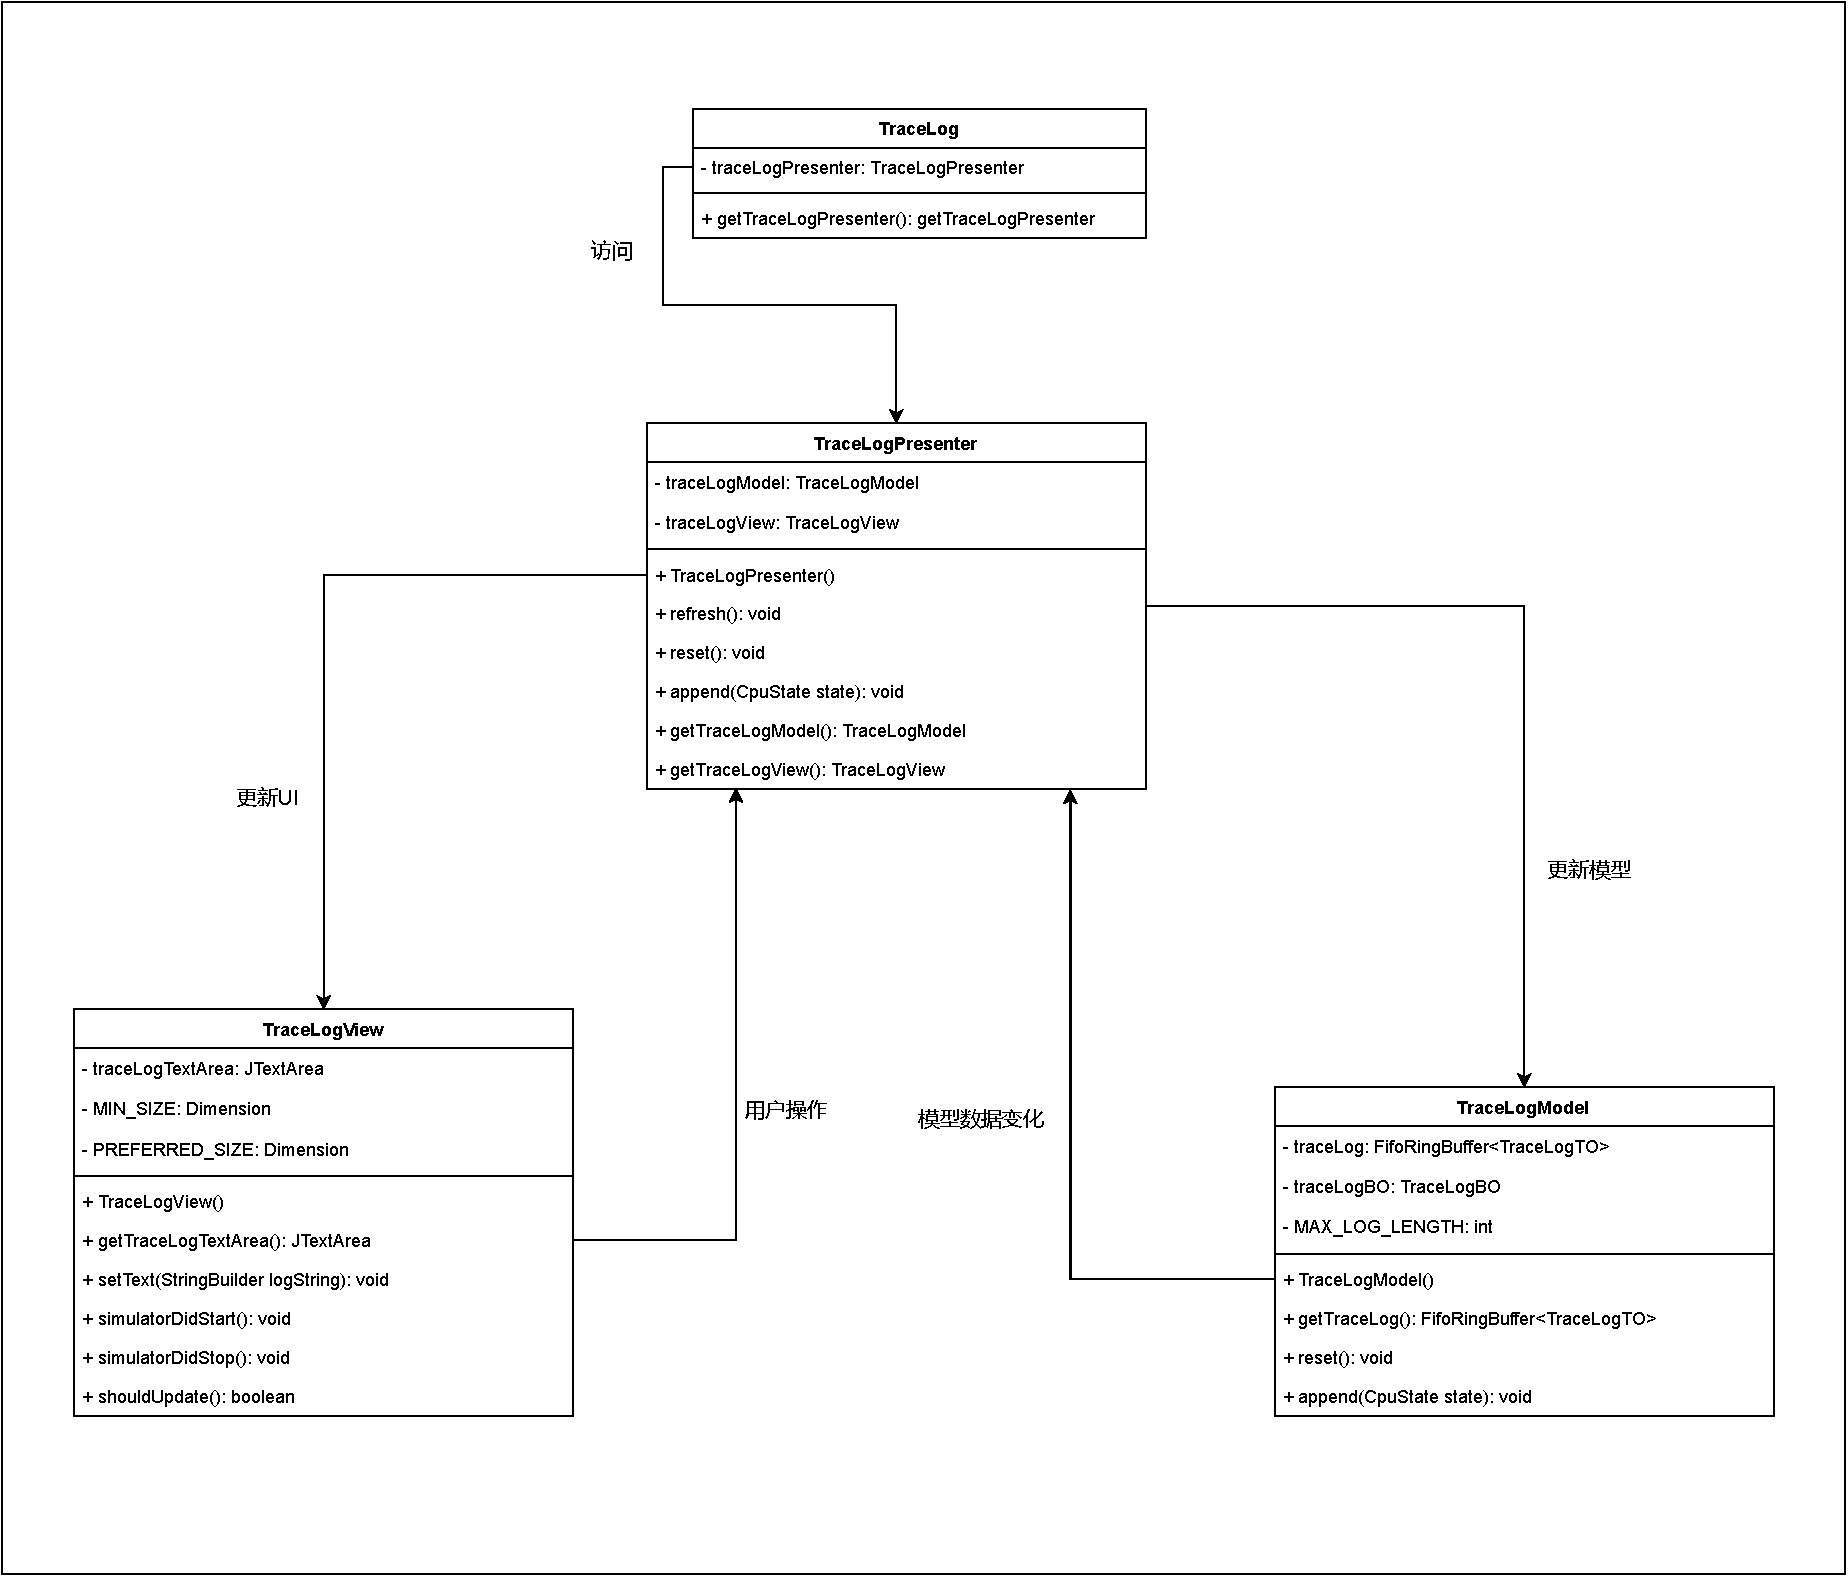
\includegraphics[width=0.9\textwidth]{figures/MVP模式.pdf}
  \caption{MVP 模式在 Slow6502 中的类图}
\end{figure}


